% Objective of the paragraph: setup the hype context and importance of the problem
Reinforcement learning (RL) is an exciting field of research as it allows for
agents to learn complex behaviors in a multitude of environments while requiring
minimal supervision in the form of reward signals. Evidence of RL's success has
accumulated in various domains ranging from playing Atari
games~\citep{MnKaSiNATURE2015} from purely visual input and defeating world GO
champions~\citep{gibney2016google}, to applications in robotic
navigation~\citep{mirowski2018learning} and
manipulation~\citep{pong2018temporal}. In the realm of multi-goal tasks, this
work introduces Floyd-Warshall Reinforcement Learning (FWRL), a new algorithm
that facilitates transferring learned behaviours in environments with dynamic
goal locations.


% brief background on model-based and model-free learning.
Algorithms in RL are often classified as being either \emph{model-based} or
\emph{model-free}, based on whether the state-transition function is learned
explicitly or implicitly~\citep{SuBaBOOK1998}.
In \emph{model-based} RL, the dynamics that govern an environment's
transitions is explicitly modelled.  At any point in an episode, agents
use this model to predict future states and utilize this information to
maximize possible reward. This formulation is known to be
sample-efficient while normally not achieving high asymptomatic
performance~\citep{pong2018temporal}.  In contrast, in \emph{model-free}
RL, algorithms such as policy gradients, actor-critic and Q-learning
directly learn the expected ``value'' for each state without explicitly
learning the environment-dynamics. This paradigm has been behind most of
the recent success stories of high performance in diverse applications
like Atari games, Go championships etc.

\begin{figure}%
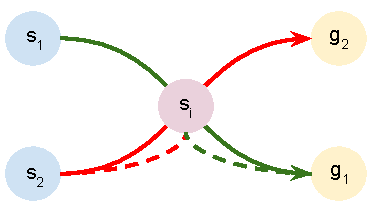
\includegraphics[width=\columnwidth]{./media/optimal_trajectories.pdf}\\
\caption{The intuition behind Floyd-Warshall Reinforcement Learning.
Consider agent gaining experience of going form $s_1$ to $g_1$ and then from
$s_2$ to $g_2$. Let's assume that there is at least one common state $s_i$ in
the two trajectories. The agent is then directed to traverse to $g_1$ from
$s_2$. The agent can use the previous trajectories to at least one path to
perform this traversal (the dotted line). However, standard Q-Learning cannot
make these generalizations. FWRL utilizes triangle-inequality like constraint
(Eq~\eqref{eq:fwconstraint}) to combine information from earlier experiences.
}
\label{fig:ql-fw-grid-world-results}%
\end{figure}

% Goal-conditioned tasks
%Many problems in robotics, like navigation, and  pick and place tasks
%can be formulated in multi-goal domains where the task to be completed
%requires the specification of goal information. However, for such tasks
In multi-goal tasks that involve static environments and dynamic goals,
such as goal-directed navigation and pick-and-place in robotics,
model-free RL struggles to transfer learned behavior from one goal
location to another within the same
environment~\citep{dhiman2018critical}. This happens because model-free
RL represents the environment as value functions which conflate the
state-dynamics and reward distributions into a single representation.
On the other hand, while model-based RL allows for the separation of
environment dynamics and reward, small errors in the modelling function
lead to significant drops in performance.

In this work we introduce Floyd-Warshall Reinforcement Learning, an
adaptation of the Floyd-Warshall shortest path
algorithm~\citep{floydwarshall1962}, for multi-goal tasks.
Floyd-Warshall shortest path algorithm is itself a generalization of
Dijkstra's algorithm in multi-goal domain on graphs. The algorithm works
by learning a a goal conditioned value function
~\citep{schaul2015universal}, called the Floyd-Warshall (FW) function,
that is defined to be the expected reward in going from a start
state-action pair $(\state, \act)$ to a given goal state $\state'$:
%
\begin{align}
\fwargs{\state}{\act}{\state'}{\policy}{} =
\E_{\policy}\left[ \sum_{t=0}^{t=k} \rew_t \middle\vert \state_0 = \state, \act_0 = \state, \state_k = \state' \right] .
\end{align}%
%
In order to learn the FW-function, we employ the following triangular-inequality constraint for shortest paths, which is our main contribution,
%
\begin{multline}
\fwargs{\state_i}{\act_i}{\state_j}{\policy^*_{\state_j}}{*}
 \ge 
  \fwargs{\state_i}{\act_i}{\state_k}{\policy^*_{\state_k}}{*}
  + \max_{\act_k}\fwargs{\state_k}{\act_k}{\state_j}{\policy^*_{\state_j}}{*}
  \\
  \forall \state_k \in \State.
  \label{eq:fwconstraint}
\end{multline}%
%
Section~\ref{sec:method} describes the terminology, equations and the method in more detail.

This constraint allows FWRL to remember paths even if they do not lead to the goal
location during particular episodes. The motivation is similar to the Hindsight
Experience Replay (HER)~\citep{anderson2017vision}, but our method allows us to
utilize hindsight experience in more fine-grained manner because we consider all
states as potential goals. Other works using goal-conditioned value function for
multi-goal tasks include Universal Value Function Approximators
(UVFA)~\citep{schaul2015universal} and Temporal Difference Models
(TDM)~\citep{pong2018temporal}. UVFA introduce goal-conditioned value functions
and a factorization approach for faster learning of neural networks that depend
upon goals from the state space. TDM combines model-based and model-free
algorithms by modeling the learning as a constrained objective function using a
horizon dependent goal-conditioned value function. In contrast, our value
function is not horizon dependent and hence has fewer parameters.


Experimentally, FWRL is shown to be more sample-efficient and achieve
higher reward standard Q-Learning, HER and model-based baselines in a
tabular setting.  FWRL is found to outperform the next most significant
baselines by as much. All code and results are made available at
\href{}{}. 


%Recently, a few works have used the idea of goal-conditioned value functions. In
%Temporal-Difference modelling \cite{pong2018temporal} model a goal conditioned
%action-value function that is also conditioned on the horizon. In contrast our
%proposed value function is independent of horizon length, and hence easier to
%estimate.



